\chapter{Introduction}
\noindent \rule{6.6in}{0.01in}
\vspace{0.2cm}

\section{Problem and Motivation}
The proliferation of Internet of Things (IoT) devices has led to a massive influx of data generated at the edge of the network \cite{mach2017mobile}. Traditional cloud computing models are increasingly inadequate to handle the strict latency and bandwidth requirements of modern real-time applications \cite{shi2016edge}. To address these challenges, Edge Computing has emerged as a paradigm shift, bringing computational resources closer to end-users.

Within the edge ecosystem, Decentralized Function-as-a-Service (DFaaS) has gained significant traction \cite{ciavotta2021edge}. DFaaS allows developers to deploy stateless micro-functions that execute on demand. However, managing highly dynamic workloads across resource-constrained edge nodes requires accurate, continuous forecasting \cite{baccarelli2017fog}. Forecasting enables proactive load balancing. Recently, Gossip Learning (GL) has been proposed to train these forecasting models across the network \cite{tundo2025decentralized}. Unlike Federated Learning, GL is fully decentralized and extremely fault-tolerant.

While Gossip Learning provides exceptional robustness, it introduces a severe inefficiency. In standard GL protocols, edge nodes blindly and continuously transmit full Machine Learning (ML) models across the network on a fixed schedule. This unchecked communication leads to massive bandwidth saturation and rapid energy depletion. Resolving this communication inefficiency is the primary motivation of this research.

\section{Problem Statement}
Standard Gossip Learning protocols exchange model updates indiscriminately, regardless of whether the transmitted model contains any statistically significant new information. This results in heavy communication overhead, redundant CPU merging cycles, and unsustainable energy drain. There is an urgent need for an adaptive mechanism that intelligently filters redundant model transmissions without degrading forecasting accuracy.

\section{Objectives}
The primary objective of this MTP is to design, implement, and validate an efficient, decentralized workload forecasting system for edge networks. 

\begin{enumerate}
    \item \textbf{To design an Adaptive Predictive-Semantic Model (APSM) filter:} Formulate a statistical threshold that dynamically suppresses redundant model transmissions based on local workload "surprise" metrics in a Gossip Learning environment.
    \item \textbf{To simulate and validate the APSM protocol:} Evaluate the proposed semantic filter using real-world Azure Serverless workload traces on a 10-node network to benchmark bandwidth reduction and MSE degradation.
\end{enumerate}

To contextualize the problem, Figure \ref{fig:intro_overview} illustrates a high-level overview of the Decentralized Edge Computing architecture. As shown, IoT devices offload real-time tasks to an interconnected mesh of Edge Nodes, which process micro-functions (DFaaS) far away from the distant Cloud Data Center. This decentralized structure necessitates peer-to-peer forecasting to prevent any single node from being overwhelmed.

\begin{figure}[!ht]
    \centering
    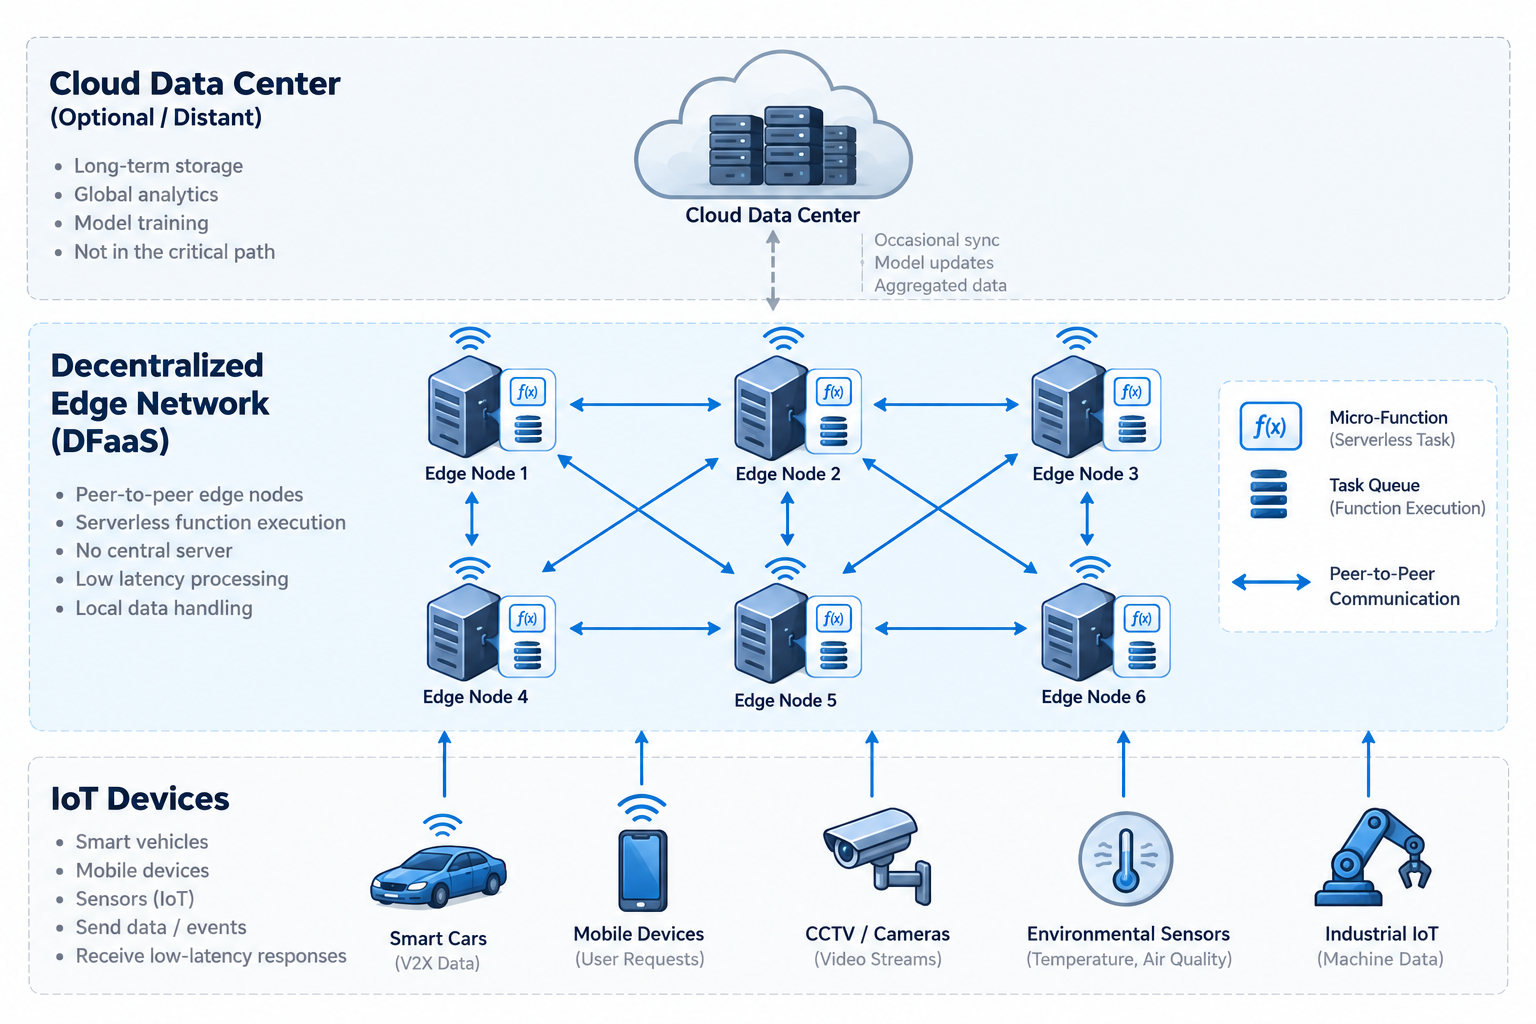
\includegraphics[width=0.6\textwidth]{chapters/figures/edge_architecture.png}
    \caption{Overview of the Decentralized Edge Computing Architecture and the DFaaS Model.}
    \label{fig:intro_overview}
\end{figure}

The remainder of this report will explore the underlying literature (Chapter 2), detail the mathematical methodology behind the APSM filter (Chapter 3), present the Phase 1 empirical results (Chapter 4), and outline the future trajectory of integrating Multi-Agent Reinforcement Learning for proactive resource orchestration (Chapter 5).
